\documentclass{beamer}

%
% Common preamble for all three parts.
%

\usepackage{xeCJK}
\setCJKmainfont{TW-Kai.ttf}
\setCJKsansfont{TW-kai.ttf}
\setCJKmonofont{TW-kai.ttf}

\usepackage[english]{babel}
\usepackage{amsmath}
\usepackage{color}
\usepackage[cache=false]{minted}
\usepackage{hyperref}
\usepackage{multicol}
\usepackage{tabularx}
\usepackage{tikz}

% only inline todonotes work
\usepackage{xkeyval}
\usepackage[textsize=small]{todonotes}
\presetkeys{todonotes}{inline}{}

\usetikzlibrary{shapes,arrows,positioning,shadows}

% no nav buttons
\usenavigationsymbolstemplate{}

\newcommand{\bftt}[1]{\textbf{\texttt{#1}}}
\newcommand{\comment}[1]{{\color[HTML]{008080}\textit{\textbf{\texttt{#1}}}}}
\newcommand{\cmd}[1]{{\color[HTML]{008000}\bftt{#1}}}
\newcommand{\bs}{\char`\\}
\newcommand{\cmdbs}[1]{\cmd{\bs#1}}
\newcommand{\lcb}{\char '173}
\newcommand{\rcb}{\char '175}
\newcommand{\cmdbegin}[1]{\cmdbs{begin\lcb}\bftt{#1}\cmd{\rcb}}
\newcommand{\cmdend}[1]{\cmdbs{end\lcb}\bftt{#1}\cmd{\rcb}}

\newcommand{\wllogo}{\textbf{Overleaf}}

% this is where the example source files are loaded from
% do not include a trailing slash
\newcommand{\fileuri}{https://raw.github.com/jdleesmiller/latex-course/master/en}

\newcommand{\wlserver}{https://www.overleaf.com}
\newcommand{\wlnewdoc}[1]{\wlserver/docs?snip\_uri=\fileuri/#1\&splash=none}

\def\tikzname{Ti\emph{k}Z}

% from http://tex.stackexchange.com/questions/5226/keyboard-font-for-latex
\newcommand*\keystroke[1]{%
  \tikz[baseline=(key.base)]
    \node[%
      draw,
      fill=white,
      drop shadow={shadow xshift=0.25ex,shadow yshift=-0.25ex,fill=black,opacity=0.75},
      rectangle,
      rounded corners=2pt,
      inner sep=1pt,
      line width=0.5pt,
      font=\scriptsize\sffamily
    ](key) {#1\strut}
  ;
}
\newcommand{\keystrokebftt}[1]{\keystroke{\bftt{#1}}}

% stolen from minted.dtx
\newenvironment{exampletwoup}
  {\VerbatimEnvironment
   \begin{VerbatimOut}{example.out}}
  {\end{VerbatimOut}
   \setlength{\parindent}{0pt}
   \fbox{\begin{tabular}{l|l}
   \begin{minipage}{0.55\linewidth}
     \inputminted[fontsize=\small,resetmargins]{latex}{example.out}
   \end{minipage} &
   \begin{minipage}{0.35\linewidth}
     \input{example.out}
   \end{minipage}
   \end{tabular}}}

\newenvironment{exampletwouptiny}
  {\VerbatimEnvironment
   \begin{VerbatimOut}{example.out}}
  {\end{VerbatimOut}
   \setlength{\parindent}{0pt}
   \fbox{\begin{tabular}{l|l}
   \begin{minipage}{0.55\linewidth}
     \inputminted[fontsize=\scriptsize,resetmargins]{latex}{example.out}
   \end{minipage} &
   \begin{minipage}{0.35\linewidth}
     \setlength{\parskip}{6pt plus 1pt minus 1pt}%
     \raggedright\scriptsize\input{example.out}
   \end{minipage}
   \end{tabular}}}

\newenvironment{exampletwouptinynoframe}
  {\VerbatimEnvironment
   \begin{VerbatimOut}{example.out}}
  {\end{VerbatimOut}
   \setlength{\parindent}{0pt}
   \begin{tabular}{l|l}
   \begin{minipage}{0.55\linewidth}
     \inputminted[fontsize=\scriptsize,resetmargins]{latex}{example.out}
   \end{minipage} &
   \begin{minipage}{0.35\linewidth}
     \setlength{\parskip}{6pt plus 1pt minus 1pt}%
     \raggedright\scriptsize\input{example.out}
   \end{minipage}
   \end{tabular}}

\title{一份互動式的\LaTeX\ 介紹}
\author{作者:Dr John D. Lees-Miller \texorpdfstring{\\[2mm]}{}
\small{譯者:周造麟}}
\titlegraphic{%

\includegraphics[height=36pt]{overleaf}\\[1em]

\includegraphics[height=24pt]{UoB-logo}
}


\subtitle{第三部:不只是文件!簡報\& 更多}

\newcommand{\alice}[1]{\todo[color=green!40]{#1}}
\newcommand{\bob}[1]{\todo[color=purple!40]{#1}}

\begin{document}

%%%%%%%%%%%%%%%%%%%%%%%%%%%%%%%%%%%%%%%%%%%%%%%%%%%%%%%%%%%%%%%%%%%%%%%%%%%%%%%
%%%%%%%%%%%%%%%%%%%%%%%%%%%%%%%%%%%%%%%%%%%%%%%%%%%%%%%%%%%%%%%%%%%%%%%%%%%%%%%
%%%%%%%%%%%%%%%%%%%%%%%%%%%%%%%%%%%%%%%%%%%%%%%%%%%%%%%%%%%%%%%%%%%%%%%%%%%%%%%
\begin{frame}
\titlepage
\end{frame}

%%%%%%%%%%%%%%%%%%%%%%%%%%%%%%%%%%%%%%%%%%%%%%%%%%%%%%%%%%%%%%%%%%%%%%%%%%%%%%%
%%%%%%%%%%%%%%%%%%%%%%%%%%%%%%%%%%%%%%%%%%%%%%%%%%%%%%%%%%%%%%%%%%%%%%%%%%%%%%%
%%%%%%%%%%%%%%%%%%%%%%%%%%%%%%%%%%%%%%%%%%%%%%%%%%%%%%%%%%%%%%%%%%%%%%%%%%%%%%%
%\begin{frame}{Setup}
%\begin{itemize}
%\item Go to this URL in Google Chrome (\emph{not} Internet Explorer) to open
%these slides on your computer:
%\vskip 2em
%\begin{center}
%\fbox{\url{http://bit.ly/12WWWqj}}
%\end{center}
%\vskip 2em
%\item Here are the slides from the previous tutorial, for reference:
%\begin{center}
%\vskip 1em
%\fbox{\href{https://dl.dropboxusercontent.com/u/31383671/site/latex_course_v2/part1.pdf}{Part 1: The Basics}}
%\vskip 1em
%\fbox{\href{https://dl.dropboxusercontent.com/u/31383671/site/latex_course_v2/part2.pdf}{Part 2: Structured Documents \& More}}
%\end{center}
%\end{itemize}
%\end{frame}

%%%%%%%%%%%%%%%%%%%%%%%%%%%%%%%%%%%%%%%%%%%%%%%%%%%%%%%%%%%%%%%%%%%%%%%%%%%%%%%
%%%%%%%%%%%%%%%%%%%%%%%%%%%%%%%%%%%%%%%%%%%%%%%%%%%%%%%%%%%%%%%%%%%%%%%%%%%%%%%
%%%%%%%%%%%%%%%%%%%%%%%%%%%%%%%%%%%%%%%%%%%%%%%%%%%%%%%%%%%%%%%%%%%%%%%%%%%%%%%
\section{回顧\LaTeX{}}

%%%%%%%%%%%%%%%%%%%%%%%%%%%%%%%%%%%%%%%%%%%%%%%%%%%%%%%%%%%%%%%%%%%%%%%%%%%%%%%
%%%%%%%%%%%%%%%%%%%%%%%%%%%%%%%%%%%%%%%%%%%%%%%%%%%%%%%%%%%%%%%%%%%%%%%%%%%%%%%
%%%%%%%%%%%%%%%%%%%%%%%%%%%%%%%%%%%%%%%%%%%%%%%%%%%%%%%%%%%%%%%%%%%%%%%%%%%%%%%
\begin{frame}[fragile]{\insertsection}
\begin{itemize}
\item 你將文件用純文字(plain text)與描述文字結構和意義的命令(\cmd{commands})
\item \texttt{latex} 將你的文字與命令轉換成格式優美的文件
\end{itemize}
\vskip 2ex
\begin{center}
\begin{minted}[frame=single]{latex}
The rain in Spain falls \emph{mainly} on the plain.
\end{minted}
\vskip 2ex
\tikz\node[single arrow,fill=gray,font=\ttfamily\bfseries,%
  rotate=270,xshift=-1em]{latex};
\vskip 2ex
\fbox{The rain in Spain falls \emph{mainly} on the plain.}
\end{center}
\end{frame}

%%%%%%%%%%%%%%%%%%%%%%%%%%%%%%%%%%%%%%%%%%%%%%%%%%%%%%%%%%%%%%%%%%%%%%%%%%%%%%%
%%%%%%%%%%%%%%%%%%%%%%%%%%%%%%%%%%%%%%%%%%%%%%%%%%%%%%%%%%%%%%%%%%%%%%%%%%%%%%%
%%%%%%%%%%%%%%%%%%%%%%%%%%%%%%%%%%%%%%%%%%%%%%%%%%%%%%%%%%%%%%%%%%%%%%%%%%%%%%%
\begin{frame}[fragile]{\insertsection{}:命令\& 參數}
\begin{itemize}
\item 命令以\emph{反斜線}開頭的\keystrokebftt{\bs}.
\item 一些命令接受在花括號 \keystrokebftt{\{}\keystrokebftt{\}}.中的\emph{參數}
\item 有些命令接受在中括號\keystrokebftt{[} \keystrokebftt{]}中的\emph{可選參數}
\vskip 2ex
\begin{exampletwouptiny}

\includegraphics[
  width=0.5\textwidth]{gerbil}


\includegraphics[
  width=0.3\textwidth,
  angle=270]{gerbil}
\end{exampletwouptiny}
\end{itemize}

\tiny{Image license: \href{https://pixabay.com/en/animal-apple-attractive-beautiful-1239390/}{CC0}}
\end{frame}

%%%%%%%%%%%%%%%%%%%%%%%%%%%%%%%%%%%%%%%%%%%%%%%%%%%%%%%%%%%%%%%%%%%%%%%%%%%%%%%
%%%%%%%%%%%%%%%%%%%%%%%%%%%%%%%%%%%%%%%%%%%%%%%%%%%%%%%%%%%%%%%%%%%%%%%%%%%%%%%
%%%%%%%%%%%%%%%%%%%%%%%%%%%%%%%%%%%%%%%%%%%%%%%%%%%%%%%%%%%%%%%%%%%%%%%%%%%%%%%
\begin{frame}[fragile]{\insertsection{}:環境}
\begin{itemize}
\item \cmdbs{begin}與\cmdbs{end}命令被用來創造許多不同的環境

\item \bftt{itemize}與\bftt{enumerate} 環境創造列表
\vskip 2ex
\begin{exampletwouptiny}
\begin{itemize} %以實心圓圈為標示
\item Biscuits
\item Tea
\end{itemize}

\begin{enumerate} %以數字為標示
\item Biscuits
\item Tea
\end{enumerate}
\end{exampletwouptiny}

\end{itemize}
\end{frame}

%%%%%%%%%%%%%%%%%%%%%%%%%%%%%%%%%%%%%%%%%%%%%%%%%%%%%%%%%%%%%%%%%%%%%%%%%%%%%%%
%%%%%%%%%%%%%%%%%%%%%%%%%%%%%%%%%%%%%%%%%%%%%%%%%%%%%%%%%%%%%%%%%%%%%%%%%%%%%%%
%%%%%%%%%%%%%%%%%%%%%%%%%%%%%%%%%%%%%%%%%%%%%%%%%%%%%%%%%%%%%%%%%%%%%%%%%%%%%%%
\begin{frame}[fragile]{\insertsection{}:數學方程式}
\begin{itemize}
\item \bftt{equation}環境創造編號過的方程式
\begin{exampletwouptiny}
\begin{equation}
  \sum_{k=1}^{n} \frac{1}{2^k}
\end{equation}
\end{exampletwouptiny}
\vskip 2ex

\item 使用錢幣符號\keystrokebftt{\$} 標記文字中的數學方程式\\[1ex]
\begin{exampletwouptiny}
% 並不是那麼好:
Let a and b be distinct positive
integers, and let c = a - b + 1.

% 好多了:
Let $a$ and $b$ be distinct positive
integers, and let $c = a - b + 1$.
\end{exampletwouptiny}
\vskip 2ex
\item 永遠記得使用一對錢幣符號 --- 一個開始一個結束
\vskip 1em
{\scriptsize 事實上\bftt{\$...\$}與\cmdbegin{math}\bftt{...}\cmdend{math}是等價的}
\end{itemize}
\end{frame}

%%%%%%%%%%%%%%%%%%%%%%%%%%%%%%%%%%%%%%%%%%%%%%%%%%%%%%%%%%%%%%%%%%%%%%%%%%%%%%%
%%%%%%%%%%%%%%%%%%%%%%%%%%%%%%%%%%%%%%%%%%%%%%%%%%%%%%%%%%%%%%%%%%%%%%%%%%%%%%%
%%%%%%%%%%%%%%%%%%%%%%%%%%%%%%%%%%%%%%%%%%%%%%%%%%%%%%%%%%%%%%%%%%%%%%%%%%%%%%%
\begin{frame}[fragile]{\insertsection{}:文件結構}
\begin{itemize}{\small
\item 以\cmdbs{documentclass}為開始 --- 文件的種類
\item 在導言區輸入重要資料(\cmdbs{title}和\cmdbs{author})還有使用的 package
\item 內容夾在\cmdbegin{document}與\cmdend{document}的中間
\item \cmdbs{maketitle}命令創造標題\cmdbs{section}創造被編號的節
}\end{itemize}
\begin{minipage}{0.55\linewidth}
\inputminted[fontsize=\scriptsize,frame=single,resetmargins]{latex}%
  {recap-structure.tex}
\end{minipage}
\begin{minipage}{0.35\linewidth}
% trim: l b r t

\includegraphics[width=\textwidth,clip,trim=1.5in 7in 3in 2in]{recap-structure.pdf}
\end{minipage}
\end{frame}

%%%%%%%%%%%%%%%%%%%%%%%%%%%%%%%%%%%%%%%%%%%%%%%%%%%%%%%%%%%%%%%%%%%%%%%%%%%%%%%
%%%%%%%%%%%%%%%%%%%%%%%%%%%%%%%%%%%%%%%%%%%%%%%%%%%%%%%%%%%%%%%%%%%%%%%%%%%%%%%
%%%%%%%%%%%%%%%%%%%%%%%%%%%%%%%%%%%%%%%%%%%%%%%%%%%%%%%%%%%%%%%%%%%%%%%%%%%%%%%
\begin{frame}[fragile]{\insertsection{}:小試身手}

\begin{enumerate}
\item 這裡有一篇短文\footnote{基於\url{http://www.cgd.ucar.edu/cms/agu/scientific_talk.html}}
\begin{center}
\fbox{\href{\wlnewdoc{recap-exercise.tex}}{%
點擊以在\wllogo{}中開啟}}
\end{center}
\vskip 2ex
\item 加一些\LaTeX{}命令,已讓他看起來像這樣:
\begin{center}
\fbox{\href{\fileuri/recap-exercise-solution.pdf}使用反斜槓(\cmdbs{\%})來讓他 \emph{跳脫}原有的意義
\item 在方程式中使用\cmdbs{frac}命令打出分數,\cmdbs{left(}和\cmdbs{right)}命令打出括號
\end{itemize}
\end{block}
\end{frame}

%%%%%%%%%%%%%%%%%%%%%%%%%%%%%%%%%%%%%%%%%%%%%%%%%%%%%%%%%%%%%%%%%%%%%%%%%%%%%%%
%%%%%%%%%%%%%%%%%%%%%%%%%%%%%%%%%%%%%%%%%%%%%%%%%%%%%%%%%%%%%%%%%%%%%%%%%%%%%%%
%%%%%%%%%%%%%%%%%%%%%%%%%%%%%%%%%%%%%%%%%%%%%%%%%%%%%%%%%%%%%%%%%%%%%%%%%%%%%%%
\section{使用\protect\bftt{beamer}製作簡報}

%%%%%%%%%%%%%%%%%%%%%%%%%%%%%%%%%%%%%%%%%%%%%%%%%%%%%%%%%%%%%%%%%%%%%%%%%%%%%%%
%%%%%%%%%%%%%%%%%%%%%%%%%%%%%%%%%%%%%%%%%%%%%%%%%%%%%%%%%%%%%%%%%%%%%%%%%%%%%%%
%%%%%%%%%%%%%%%%%%%%%%%%%%%%%%%%%%%%%%%%%%%%%%%%%%%%%%%%%%%%%%%%%%%%%%%%%%%%%%%
\begin{frame}[fragile]{\insertsection}
\begin{itemize}
\item Beamer是用來製作簡報的\LaTeX{} package (就像這個)
\item 它提供了文件類型:\bftt{beamer}
\item 使用\bftt{frame}環境製作投影片
\end{itemize}
\begin{minipage}{0.55\linewidth}
\inputminted[fontsize=\scriptsize,frame=single,resetmargins]{latex}%
  {beamer-minimal.tex}
\end{minipage}
\begin{minipage}{0.35\linewidth}
% trim: l b r t

\includegraphics[width=\textwidth,clip,trim=1in 1in 1in 1in]{beamer-minimal.pdf}
\end{minipage}
\end{frame}

%%%%%%%%%%%%%%%%%%%%%%%%%%%%%%%%%%%%%%%%%%%%%%%%%%%%%%%%%%%%%%%%%%%%%%%%%%%%%%%
%%%%%%%%%%%%%%%%%%%%%%%%%%%%%%%%%%%%%%%%%%%%%%%%%%%%%%%%%%%%%%%%%%%%%%%%%%%%%%%
%%%%%%%%%%%%%%%%%%%%%%%%%%%%%%%%%%%%%%%%%%%%%%%%%%%%%%%%%%%%%%%%%%%%%%%%%%%%%%%
\label{待翻譯}
\begin{frame}[fragile]{\insertsection{}:Following Along}

\begin{itemize}
\item As we go through the following slides, try out the examples by typing them
into the example document on \wllogo.
\end{itemize}
\vskip 2ex
\begin{center}
\fbox{\href{\wlnewdoc{beamer-minimal.tex}}{%
Click to open the example document in \wllogo{}}}
\end{center}
\end{frame}

%%%%%%%%%%%%%%%%%%%%%%%%%%%%%%%%%%%%%%%%%%%%%%%%%%%%%%%%%%%%%%%%%%%%%%%%%%%%%%%
%%%%%%%%%%%%%%%%%%%%%%%%%%%%%%%%%%%%%%%%%%%%%%%%%%%%%%%%%%%%%%%%%%%%%%%%%%%%%%%
%%%%%%%%%%%%%%%%%%%%%%%%%%%%%%%%%%%%%%%%%%%%%%%%%%%%%%%%%%%%%%%%%%%%%%%%%%%%%%%
\begin{frame}[fragile]
\frametitle{\insertsection:Frames環境}
\begin{itemize}
\item 使用\cmdbs{frametitle}賦予投影片標題
\item 然後把內容打在Frames環境中
\item 這張投影片的原始碼如下:
\vskip 2ex
\inputminted[fontsize=\scriptsize,frame=single,resetmargins]{latex}%
  {beamer-frame.tex}
\end{itemize}
\end{frame}

%%%%%%%%%%%%%%%%%%%%%%%%%%%%%%%%%%%%%%%%%%%%%%%%%%%%%%%%%%%%%%%%%%%%%%%%%%%%%%%
%%%%%%%%%%%%%%%%%%%%%%%%%%%%%%%%%%%%%%%%%%%%%%%%%%%%%%%%%%%%%%%%%%%%%%%%%%%%%%%
%%%%%%%%%%%%%%%%%%%%%%%%%%%%%%%%%%%%%%%%%%%%%%%%%%%%%%%%%%%%%%%%%%%%%%%%%%%%%%%
\begin{frame}[fragile]{\insertsection:節}
\begin{itemize}
\item 你可以使用\cmdbs{section}將\bftt{frame}分組\bftt{beamer}可以利用他們自動產生大綱
\item 使用\cmdbs{tableofcontents}來產生大綱,\bftt{currentsection}選項強調現在所在的section
\vskip 2ex
\begin{exampletwouptiny}
\tableofcontents[currentsection]
\end{exampletwouptiny}
\end{itemize}
\end{frame}

%%%%%%%%%%%%%%%%%%%%%%%%%%%%%%%%%%%%%%%%%%%%%%%%%%%%%%%%%%%%%%%%%%%%%%%%%%%%%%%
%%%%%%%%%%%%%%%%%%%%%%%%%%%%%%%%%%%%%%%%%%%%%%%%%%%%%%%%%%%%%%%%%%%%%%%%%%%%%%%
%%%%%%%%%%%%%%%%%%%%%%%%%%%%%%%%%%%%%%%%%%%%%%%%%%%%%%%%%%%%%%%%%%%%%%%%%%%%%%%
\begin{frame}[fragile]{\insertsection:多欄}
\begin{columns}
\begin{column}{0.4\textwidth}
\begin{itemize}
\item 使用\bftt{columns}和\bftt{column}環境將投影片分欄
\item \bftt{column}的參數決定了該欄的寬度
\item 也可以去看看\bftt{multicol} package,他會自動將你的內容分欄
\end{itemize}
\end{column}
\begin{column}{0.6\textwidth}
\begin{minted}[fontsize=\scriptsize,frame=single]{latex}
\begin{columns}
  \begin{column}{0.4\textwidth}
    \begin{itemize}
    \item 使用\bftt{columns} ...
    \item \bftt{column}的參數 ...
    \item 也可以去看看 ...
    \end{itemize}
  \end{column}
  \begin{column}{0.6\textwidth}
    % 第二欄
  \end{column}
\end{columns}
\end{minted}
\end{column}
\end{columns}
\end{frame}

%%%%%%%%%%%%%%%%%%%%%%%%%%%%%%%%%%%%%%%%%%%%%%%%%%%%%%%%%%%%%%%%%%%%%%%%%%%%%%%
%%%%%%%%%%%%%%%%%%%%%%%%%%%%%%%%%%%%%%%%%%%%%%%%%%%%%%%%%%%%%%%%%%%%%%%%%%%%%%%
%%%%%%%%%%%%%%%%%%%%%%%%%%%%%%%%%%%%%%%%%%%%%%%%%%%%%%%%%%%%%%%%%%%%%%%%%%%%%%%
\begin{frame}[fragile]{\insertsection:強調}
\begin{itemize}

\item 使用\cmdbs{emph}或\cmdbs{alert}來強調:
\vskip 1ex
\begin{exampletwouptiny}
I should \emph{emphasise} that
this is an \alert{important} point.
\end{exampletwouptiny}
\vskip 1ex

\item 或使用粗體和斜體
\vskip 1ex
\begin{exampletwouptiny}
Text in \textbf{bold face}.
Text in \textit{italics}.
\end{exampletwouptiny}
\vskip 1ex

\item 或使用顏色:
\vskip 1ex
\begin{exampletwouptiny}
It \textcolor{red}{stops}
and \textcolor{green}{starts}.
\end{exampletwouptiny}
\vskip 1ex
\item 在\url{http://www.math.umbc.edu/~rouben/beamer/quickstart-Z-H-25.html}找到更多顏色或自定義顏色
\end{itemize}
\end{frame}

%%%%%%%%%%%%%%%%%%%%%%%%%%%%%%%%%%%%%%%%%%%%%%%%%%%%%%%%%%%%%%%%%%%%%%%%%%%%%%%
%%%%%%%%%%%%%%%%%%%%%%%%%%%%%%%%%%%%%%%%%%%%%%%%%%%%%%%%%%%%%%%%%%%%%%%%%%%%%%%
%%%%%%%%%%%%%%%%%%%%%%%%%%%%%%%%%%%%%%%%%%%%%%%%%%%%%%%%%%%%%%%%%%%%%%%%%%%%%%%
\begin{frame}[fragile]{\insertsection:圖片}
\begin{itemize}
\item 使用\bftt{graphicx} package提供的\cmdbs{includegraphics}命令
\item \bftt{figure}環境在\bftt{beamer}中預設為置中
\vskip 2ex
\begin{exampletwouptiny}
\begin{figure}

\includegraphics[
  width=0.5\textwidth]{gerbil}
\end{figure}
\end{exampletwouptiny}
\end{itemize}

\tiny{Image license: \href{https://pixabay.com/en/animal-apple-attractive-beautiful-1239390/}{CC0}}
\end{frame}

%%%%%%%%%%%%%%%%%%%%%%%%%%%%%%%%%%%%%%%%%%%%%%%%%%%%%%%%%%%%%%%%%%%%%%%%%%%%%%%
%%%%%%%%%%%%%%%%%%%%%%%%%%%%%%%%%%%%%%%%%%%%%%%%%%%%%%%%%%%%%%%%%%%%%%%%%%%%%%%
%%%%%%%%%%%%%%%%%%%%%%%%%%%%%%%%%%%%%%%%%%%%%%%%%%%%%%%%%%%%%%%%%%%%%%%%%%%%%%%
\begin{frame}[fragile]{\insertsection:表格}
\begin{itemize}
\item 在\LaTeX{}中使用表格需經過一番適應
\item 使用\bftt{tabularx} package 提供的\bftt{tabular}環境
\item 指定表格靠齊位置的參數 --- \textbf{l}eft, \textbf{r}ight, \textbf{r}ight.
\begin{exampletwouptiny}
\begin{tabular}{lrr}
Item   & Qty & Unit \$ \\
Widget & 1   & 199.99  \\
Gadget & 2   & 399.99  \\
Cable  & 3   & 19.99   \\
\end{tabular}
\end{exampletwouptiny}
\item 這同時也可以指定表格中的垂直線,使用\cmdbs{hline}命令指定水平線
\begin{exampletwouptiny}
\begin{tabular}{|l|r|r|} \hline
Item   & Qty & Unit \$ \\\hline
Widget & 1   & 199.99  \\
Gadget & 2   & 399.99  \\
Cable  & 3   & 19.99   \\\hline
\end{tabular}
\end{exampletwouptiny}
\item 使用與號\keystrokebftt{\&}來接每一格分開,使用雙重反斜槓\keystrokebftt{\bs}\keystrokebftt{\bs}來換行(就像 part 1 中提過的\bftt{align*}環境)
\end{itemize}
\end{frame}

%%%%%%%%%%%%%%%%%%%%%%%%%%%%%%%%%%%%%%%%%%%%%%%%%%%%%%%%%%%%%%%%%%%%%%%%%%%%%%%
%%%%%%%%%%%%%%%%%%%%%%%%%%%%%%%%%%%%%%%%%%%%%%%%%%%%%%%%%%%%%%%%%%%%%%%%%%%%%%%
%%%%%%%%%%%%%%%%%%%%%%%%%%%%%%%%%%%%%%%%%%%%%%%%%%%%%%%%%%%%%%%%%%%%%%%%%%%%%%%
\begin{frame}[fragile]{\insertsection:Blocks}
\begin{itemize}
\item \bftt{block}環境製造有標題的箱子
\begin{exampletwouptiny}
\begin{block}{有趣的事實}
這很重要!
\end{block}

\begin{alertblock}{警世故事}
這真的超重要!!!
\end{alertblock}
\end{exampletwouptiny}

\item 箱子的外型取決於beamer的主題\ldots
\end{itemize}
\end{frame}

%%%%%%%%%%%%%%%%%%%%%%%%%%%%%%%%%%%%%%%%%%%%%%%%%%%%%%%%%%%%%%%%%%%%%%%%%%%%%%%
%%%%%%%%%%%%%%%%%%%%%%%%%%%%%%%%%%%%%%%%%%%%%%%%%%%%%%%%%%%%%%%%%%%%%%%%%%%%%%%
%%%%%%%%%%%%%%%%%%%%%%%%%%%%%%%%%%%%%%%%%%%%%%%%%%%%%%%%%%%%%%%%%%%%%%%%%%%%%%%
\begin{frame}[fragile]
\frametitle{\insertsection:主題}
\begin{itemize}
\item 使用主題自定義報告的外觀
\item 在\url{http://deic.uab.es/~iblanes/beamer_gallery/index_by_theme.html}可以找到大量的主題%for a large collection of themes
\end{itemize}
\begin{minipage}{0.55\linewidth}
\inputminted[fontsize=\scriptsize,frame=single,resetmargins]{latex}%
  {beamer-theme.tex}
\end{minipage}
\begin{minipage}{0.35\linewidth}
% trim: l b r t

\includegraphics[width=\textwidth]{beamer-theme.pdf}
\end{minipage}
\end{frame}

%%%%%%%%%%%%%%%%%%%%%%%%%%%%%%%%%%%%%%%%%%%%%%%%%%%%%%%%%%%%%%%%%%%%%%%%%%%%%%%
%%%%%%%%%%%%%%%%%%%%%%%%%%%%%%%%%%%%%%%%%%%%%%%%%%%%%%%%%%%%%%%%%%%%%%%%%%%%%%%
%%%%%%%%%%%%%%%%%%%%%%%%%%%%%%%%%%%%%%%%%%%%%%%%%%%%%%%%%%%%%%%%%%%%%%%%%%%%%%%
\begin{frame}[fragile]{\insertsection:動畫}
\begin{itemize}
\item 一個frame可以產生許多投影片
\item 使用\cmdbs{pause}命令將投影片內容分開
\vskip 2ex
\begin{exampletwouptinynoframe}
\begin{itemize}
\item 你感受到
\pause \item 暫停了嗎?
\end{itemize}
\end{exampletwouptinynoframe}
\vskip 2ex
\item 更多巧妙的\bftt{beamer}動畫:參考\cmdbs{only}, \cmdbs{alt}和 \cmdbs{uncover}命令%There many more clever ways of making animations in beamer; see also the \only, \alt, and \uncover commands.
\label{待翻譯}
\end{itemize}
\end{frame}

%%%%%%%%%%%%%%%%%%%%%%%%%%%%%%%%%%%%%%%%%%%%%%%%%%%%%%%%%%%%%%%%%%%%%%%%%%%%%%%
%%%%%%%%%%%%%%%%%%%%%%%%%%%%%%%%%%%%%%%%%%%%%%%%%%%%%%%%%%%%%%%%%%%%%%%%%%%%%%%
%%%%%%%%%%%%%%%%%%%%%%%%%%%%%%%%%%%%%%%%%%%%%%%%%%%%%%%%%%%%%%%%%%%%%%%%%%%%%%%
\begin{frame}[fragile]{\insertsection:小試身手}

將Peter Norvig's excellent 的``Gettysburg Powerpoint Presentation''利用 \bftt{beamer}重置\footnote{\url{http://norvig.com/Gettysburg}}

\begin{enumerate}
\item 在\wllogo{}打開練習:
\begin{center}
\fbox{\href{\wlnewdoc{beamer-exercise.tex}}{%
點擊以在\wllogo{}中開啟}}
\end{center}
\vskip 2ex
\item 將範例圖片下載到你的電腦裡面,再用files menu將圖片上傳到\wllogo{}
\begin{center}
\fbox{\href{\fileuri/gettysburg_graph.png?dl=1}{點擊以下載圖片}}
\end{center}
\vskip 2ex
\item 加入\LaTeX{}命令使他看起來像範例
\begin{center}
\fbox{\href{\fileuri/beamer-exercise-solution.pdf}{%
點擊以下載範例檔案}}
\end{center}
\end{enumerate}
\end{frame}

%%%%%%%%%%%%%%%%%%%%%%%%%%%%%%%%%%%%%%%%%%%%%%%%%%%%%%%%%%%%%%%%%%%%%%%%%%%%%%%
%%%%%%%%%%%%%%%%%%%%%%%%%%%%%%%%%%%%%%%%%%%%%%%%%%%%%%%%%%%%%%%%%%%%%%%%%%%%%%%
%%%%%%%%%%%%%%%%%%%%%%%%%%%%%%%%%%%%%%%%%%%%%%%%%%%%%%%%%%%%%%%%%%%%%%%%%%%%%%%
\section{利用\protect\tikzname{}畫畫}

%%%%%%%%%%%%%%%%%%%%%%%%%%%%%%%%%%%%%%%%%%%%%%%%%%%%%%%%%%%%%%%%%%%%%%%%%%%%%%%
%%%%%%%%%%%%%%%%%%%%%%%%%%%%%%%%%%%%%%%%%%%%%%%%%%%%%%%%%%%%%%%%%%%%%%%%%%%%%%%
%%%%%%%%%%%%%%%%%%%%%%%%%%%%%%%%%%%%%%%%%%%%%%%%%%%%%%%%%%%%%%%%%%%%%%%%%%%%%%%
\begin{frame}[fragile]{\insertsection}
\begin{itemize}
\item \tikzname{}是個用來畫畫的\LaTeX{}package
\item 他在\LaTeX{}中定義了強大繪圖語言,簡單的程式碼就可以創造讓人驚豔的圖片
\begin{figure}
\href{http://www.texample.net/tikz/examples/rotated-triangle/}{%
  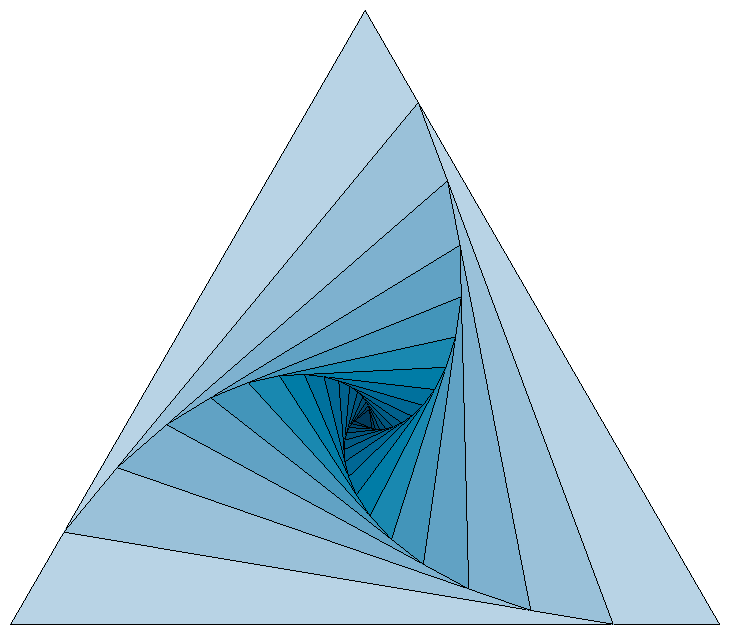
\includegraphics[width=0.35\textwidth]{rotated-triangle}}
\end{figure}
\item 我們會從簡單的事物開始,在\tikzname{}中畫直線:
\vskip 1ex
\begin{exampletwouptiny}
\begin{tikzpicture}
\draw (0,0) -- (1,1); % 一條線
\end{tikzpicture}
\end{exampletwouptiny}
\end{itemize}
\end{frame}

%%%%%%%%%%%%%%%%%%%%%%%%%%%%%%%%%%%%%%%%%%%%%%%%%%%%%%%%%%%%%%%%%%%%%%%%%%%%%%%
%%%%%%%%%%%%%%%%%%%%%%%%%%%%%%%%%%%%%%%%%%%%%%%%%%%%%%%%%%%%%%%%%%%%%%%%%%%%%%%
%%%%%%%%%%%%%%%%%%%%%%%%%%%%%%%%%%%%%%%%%%%%%%%%%%%%%%%%%%%%%%%%%%%%%%%%%%%%%%%
\begin{frame}[fragile]{\insertsection:座標}
\begin{itemize}
\item 預設的座標單位是公分:
\begin{figure}
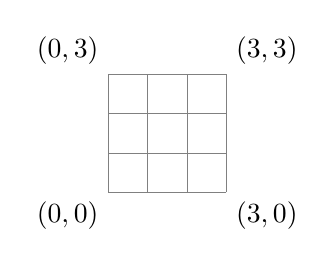
\begin{tikzpicture}[scale=0.5]
\draw[help lines] (0,0) grid (3,3);
\node[below left] at (0,0) {$(0,0)$};
\node[below right] at (3,0) {$(3,0)$};
\node[above right] at (3,3) {$(3,3)$};
\node[above left] at (0,3) {$(0,3)$};
\end{tikzpicture}
\end{figure}
\item 在使用\tikzname{}時畫一個網格是個好主意:
\vskip 1ex
\begin{exampletwouptiny}

\begin{tikzpicture}
\draw[help lines] (0,0) grid (3,3);
\end{tikzpicture}
\end{exampletwouptiny}
\end{itemize}
\end{frame}

%%%%%%%%%%%%%%%%%%%%%%%%%%%%%%%%%%%%%%%%%%%%%%%%%%%%%%%%%%%%%%%%%%%%%%%%%%%%%%%
%%%%%%%%%%%%%%%%%%%%%%%%%%%%%%%%%%%%%%%%%%%%%%%%%%%%%%%%%%%%%%%%%%%%%%%%%%%%%%%
%%%%%%%%%%%%%%%%%%%%%%%%%%%%%%%%%%%%%%%%%%%%%%%%%%%%%%%%%%%%%%%%%%%%%%%%%%%%%%%
\begin{frame}[fragile]{\insertsection:直線}
\begin{itemize}
\item 箭頭與線條格式是\cmdbs{draw}的可選參數
\item 每一個draw命令後都用分號\keystrokebftt{;}來結束
\vskip 1ex
\begin{exampletwouptiny}
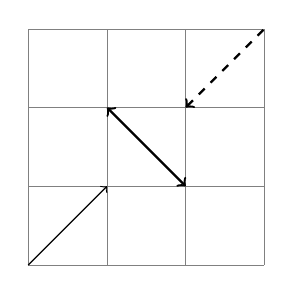
\begin{tikzpicture}
\draw[help lines] (0,0) grid (3,3);
\draw[->] (0,0) -- (1,1);
\draw[<->, thick] (2,1) -- (1,2);
\draw[<-, thick, dashed] (2,2)--(3,3);
\end{tikzpicture}
\end{exampletwouptiny}
\end{itemize}
\end{frame}

%%%%%%%%%%%%%%%%%%%%%%%%%%%%%%%%%%%%%%%%%%%%%%%%%%%%%%%%%%%%%%%%%%%%%%%%%%%%%%%
%%%%%%%%%%%%%%%%%%%%%%%%%%%%%%%%%%%%%%%%%%%%%%%%%%%%%%%%%%%%%%%%%%%%%%%%%%%%%%%
%%%%%%%%%%%%%%%%%%%%%%%%%%%%%%%%%%%%%%%%%%%%%%%%%%%%%%%%%%%%%%%%%%%%%%%%%%%%%%%
\begin{frame}[fragile]{\insertsection:路徑}
\begin{itemize}
\item 你可以指定多個點來形成一條路徑
\item 箭頭只會在路徑的終點出現
\vskip 1ex
\begin{exampletwouptiny}
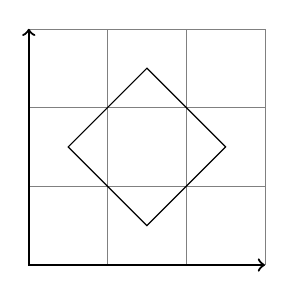
\begin{tikzpicture}
\draw[help lines] (0,0) grid (3,3);
% 座標軸
\draw[<->, thick] (0,3)--(0,0)--(3,0);
% 鑽石
\draw (1.5,0.5) -- (2.5,1.5) -- 
      (1.5,2.5) -- (0.5,1.5) --
      cycle; % 封閉路徑
\end{tikzpicture}
\end{exampletwouptiny}
\end{itemize}
\end{frame}

%%%%%%%%%%%%%%%%%%%%%%%%%%%%%%%%%%%%%%%%%%%%%%%%%%%%%%%%%%%%%%%%%%%%%%%%%%%%%%%
%%%%%%%%%%%%%%%%%%%%%%%%%%%%%%%%%%%%%%%%%%%%%%%%%%%%%%%%%%%%%%%%%%%%%%%%%%%%%%%
%%%%%%%%%%%%%%%%%%%%%%%%%%%%%%%%%%%%%%%%%%%%%%%%%%%%%%%%%%%%%%%%%%%%%%%%%%%%%%%
\begin{frame}[fragile]{\insertsection:顏色}
\begin{itemize}
\item 箭頭與線條格式也是\cmdbs{draw}的可選參數
\vskip 1ex
\begin{exampletwouptiny}
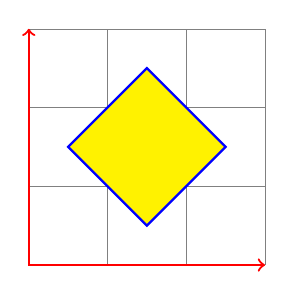
\begin{tikzpicture}
\draw[help lines] (0,0) grid (3,3);
% 座標軸
\draw[<->, thick, red]
  (0,3)--(0,0)--(3,0); 
% 鑽石
\draw[thick, blue, fill=yellow]
  (1.5,0.5) -- (2.5,1.5) -- 
  (1.5,2.5) -- (0.5,1.5) --
  cycle;
\end{tikzpicture}
\end{exampletwouptiny}
\end{itemize}
\end{frame}

%%%%%%%%%%%%%%%%%%%%%%%%%%%%%%%%%%%%%%%%%%%%%%%%%%%%%%%%%%%%%%%%%%%%%%%%%%%%%%%
%%%%%%%%%%%%%%%%%%%%%%%%%%%%%%%%%%%%%%%%%%%%%%%%%%%%%%%%%%%%%%%%%%%%%%%%%%%%%%%
%%%%%%%%%%%%%%%%%%%%%%%%%%%%%%%%%%%%%%%%%%%%%%%%%%%%%%%%%%%%%%%%%%%%%%%%%%%%%%%
\begin{frame}[fragile]{\insertsection:形狀}
\begin{itemize}
\item \tikzname{}內建了指令來畫出簡單圖形
\vskip 1ex
\begin{exampletwouptiny}
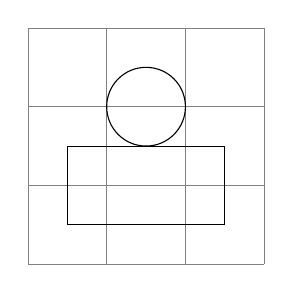
\begin{tikzpicture}
\draw[help lines] (0,0) grid (3,3);
\draw (1.5,2.0) circle (0.5);
\draw (0.5,0.5) rectangle (2.5,1.5);
\end{tikzpicture}
\end{exampletwouptiny}
\end{itemize}
\end{frame}

%%%%%%%%%%%%%%%%%%%%%%%%%%%%%%%%%%%%%%%%%%%%%%%%%%%%%%%%%%%%%%%%%%%%%%%%%%%%%%%
%%%%%%%%%%%%%%%%%%%%%%%%%%%%%%%%%%%%%%%%%%%%%%%%%%%%%%%%%%%%%%%%%%%%%%%%%%%%%%%
%%%%%%%%%%%%%%%%%%%%%%%%%%%%%%%%%%%%%%%%%%%%%%%%%%%%%%%%%%%%%%%%%%%%%%%%%%%%%%%
\begin{frame}[fragile]{\insertsection:節點 \& 標籤}
\begin{itemize}
\item 在\tikzname{}圖畫中,使用節點來放置文字(還有數學方程式)
\item 你也可以將節點當作座標點來使用 --- 對圖表很有用
\vskip 1ex
\begin{exampletwouptiny}
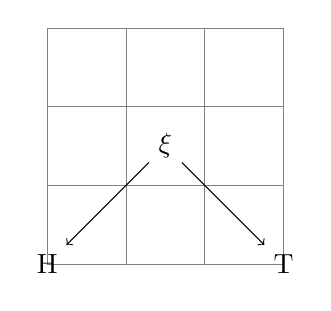
\begin{tikzpicture}
\draw[help lines] (0,0) grid (3,3);
\node (h) at (0,0) {H};
\node (x) at (1.5,1.5) {$\xi$};
\node (t) at (3,0) {T};
\draw[->] (x) -- (h);
\draw[->] (x) -- (t);
\end{tikzpicture}
\end{exampletwouptiny}
\end{itemize}
\end{frame}

%%%%%%%%%%%%%%%%%%%%%%%%%%%%%%%%%%%%%%%%%%%%%%%%%%%%%%%%%%%%%%%%%%%%%%%%%%%%%%%
%%%%%%%%%%%%%%%%%%%%%%%%%%%%%%%%%%%%%%%%%%%%%%%%%%%%%%%%%%%%%%%%%%%%%%%%%%%%%%%
%%%%%%%%%%%%%%%%%%%%%%%%%%%%%%%%%%%%%%%%%%%%%%%%%%%%%%%%%%%%%%%%%%%%%%%%%%%%%%%
\begin{frame}[fragile]{\insertsection:函數}
\begin{itemize}
\item 你甚至可以畫出一些簡單的函數圖形
\vskip 1ex
\begin{exampletwouptiny}
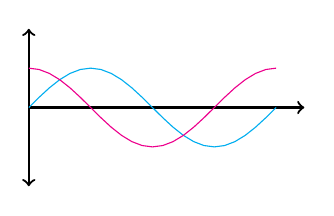
\begin{tikzpicture}[scale=0.5]
% y 軸
\draw[<->, thick] (0,2) -- (0,-2);
% x 軸
\draw[ ->, thick] (0,0) -- (7, 0); 
% 曲線
\draw[cyan,domain=0:2*pi]
  plot (\x, {sin(\x r)});
\draw[magenta,domain=0:2*pi]
  plot (\x, {cos(\x r)});
\end{tikzpicture}
\end{exampletwouptiny}
\end{itemize}
\end{frame}

%%%%%%%%%%%%%%%%%%%%%%%%%%%%%%%%%%%%%%%%%%%%%%%%%%%%%%%%%%%%%%%%%%%%%%%%%%%%%%%
%%%%%%%%%%%%%%%%%%%%%%%%%%%%%%%%%%%%%%%%%%%%%%%%%%%%%%%%%%%%%%%%%%%%%%%%%%%%%%%
%%%%%%%%%%%%%%%%%%%%%%%%%%%%%%%%%%%%%%%%%%%%%%%%%%%%%%%%%%%%%%%%%%%%%%%%%%%%%%%
\begin{frame}[fragile]{\insertsection:更多例子}
\begin{itemize}
\item 想要更多\tikzname{}的例子嗎?查看 \fbox{\href{http://texample.net/tikz/}{\TeX{}ample.net}}
\end{itemize}
\begin{figure}
\href{http://texample.net/tikz/examples/escher-brick-penrose-triangle/}{%
  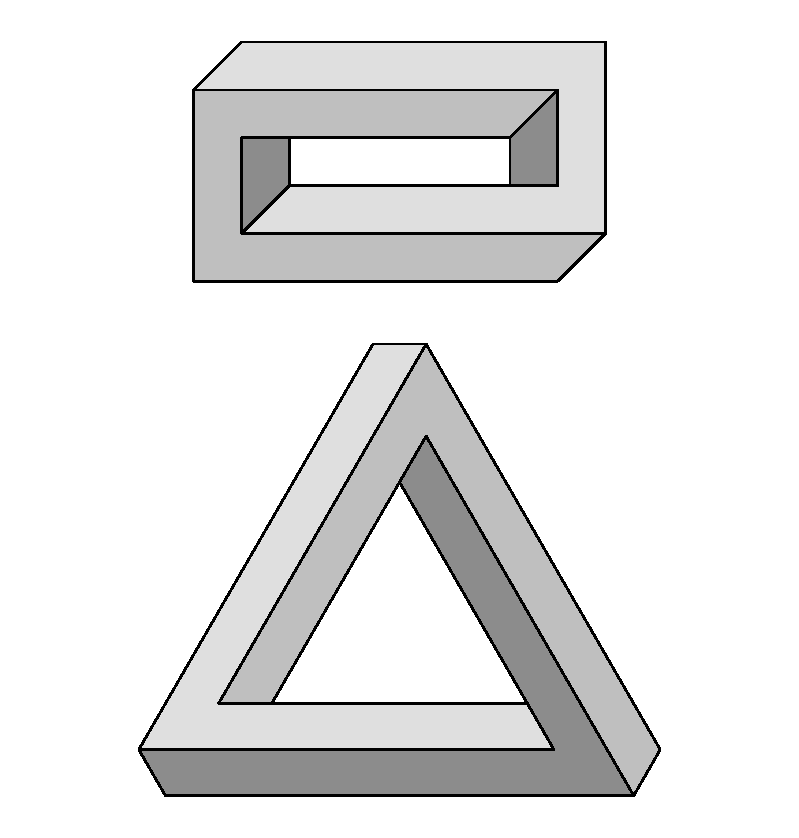
\includegraphics[width=0.3\textwidth]{escher-brick-penrose-triangle}}
\href{http://texample.net/tikz/examples/computer-science-mindmap/}{%
  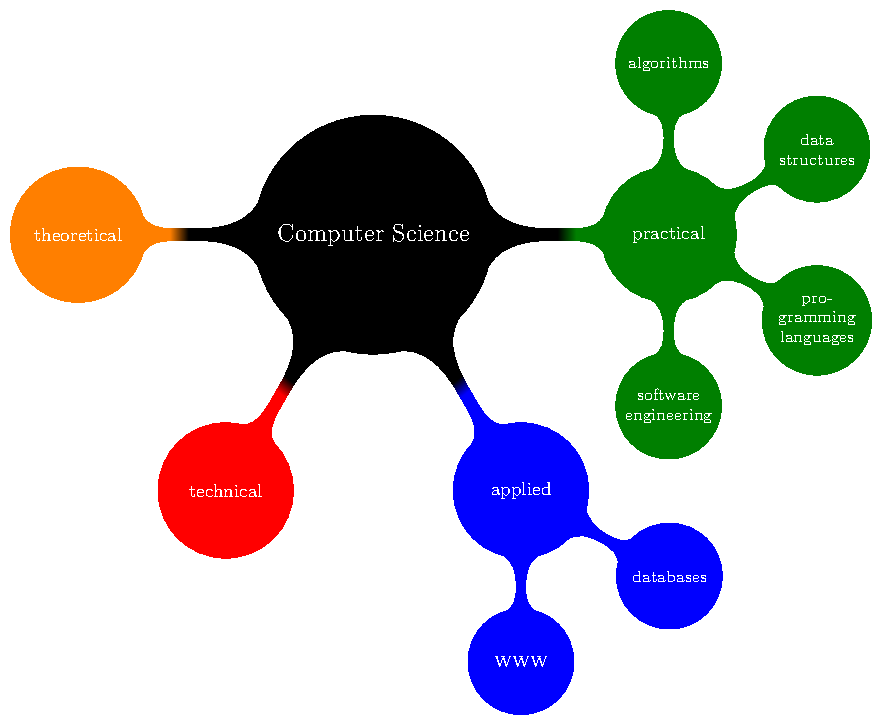
\includegraphics[width=0.3\textwidth]{computer-science-mindmap}}
\href{http://texample.net/tikz/examples/gajski-kuhn-y-chart/}{%
  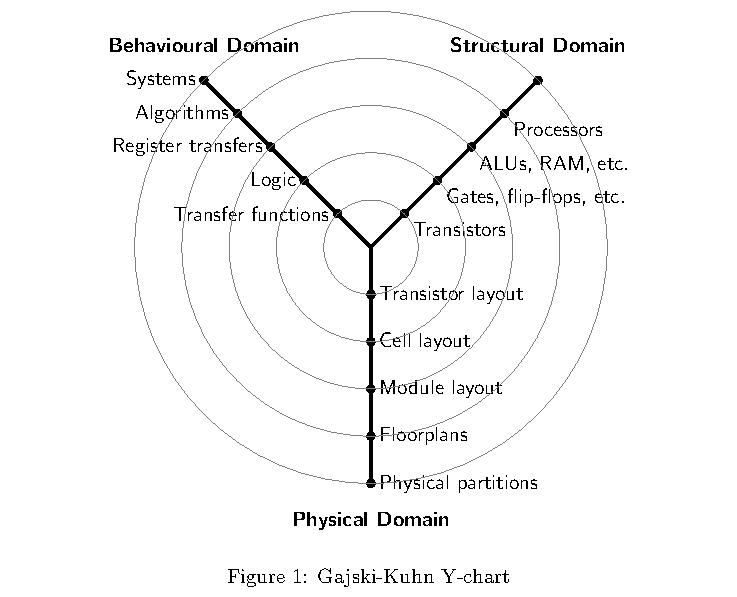
\includegraphics[width=0.3\textwidth]{gajski-kuhn-y-chart}}
\end{figure}
\end{frame}

%%%%%%%%%%%%%%%%%%%%%%%%%%%%%%%%%%%%%%%%%%%%%%%%%%%%%%%%%%%%%%%%%%%%%%%%%%%%%%%
%%%%%%%%%%%%%%%%%%%%%%%%%%%%%%%%%%%%%%%%%%%%%%%%%%%%%%%%%%%%%%%%%%%%%%%%%%%%%%%
%%%%%%%%%%%%%%%%%%%%%%%%%%%%%%%%%%%%%%%%%%%%%%%%%%%%%%%%%%%%%%%%%%%%%%%%%%%%%%%
\begin{frame}[fragile]{\insertsection:小試身手}
利用\tikzname{}畫出這個:\footnote{基於\url{http://xkcd.com/1022}}
\begin{figure}
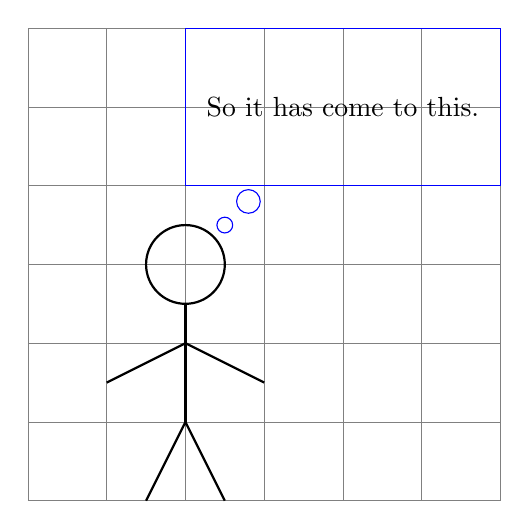
\begin{tikzpicture}
\draw[help lines] (0,0) grid (6,6);
\draw[thick] (2,3) circle (0.5);
\draw[thick] (2,2.5) -- (2,1);              % body
\draw[thick] (1,1.5) -- (2,2) -- (3,1.5);   % arms
\draw[thick] (1.5, 0) -- (2,1) -- (2.5, 0); % legs
\draw[blue] (2,4) rectangle (6,6);
\draw[blue] (2.5,3.5) circle (0.1);
\draw[blue] (2.8,3.8) circle (0.15);
\node at (4,5) {So it has come to this.};
\end{tikzpicture}

\end{figure}
\end{frame}

%%%%%%%%%%%%%%%%%%%%%%%%%%%%%%%%%%%%%%%%%%%%%%%%%%%%%%%%%%%%%%%%%%%%%%%%%%%%%%%
%%%%%%%%%%%%%%%%%%%%%%%%%%%%%%%%%%%%%%%%%%%%%%%%%%%%%%%%%%%%%%%%%%%%%%%%%%%%%%%
%%%%%%%%%%%%%%%%%%%%%%%%%%%%%%%%%%%%%%%%%%%%%%%%%%%%%%%%%%%%%%%%%%%%%%%%%%%%%%%
\section{註釋:\protect\bftt{todonotes}}

%%%%%%%%%%%%%%%%%%%%%%%%%%%%%%%%%%%%%%%%%%%%%%%%%%%%%%%%%%%%%%%%%%%%%%%%%%%%%%%
%%%%%%%%%%%%%%%%%%%%%%%%%%%%%%%%%%%%%%%%%%%%%%%%%%%%%%%%%%%%%%%%%%%%%%%%%%%%%%%
%%%%%%%%%%%%%%%%%%%%%%%%%%%%%%%%%%%%%%%%%%%%%%%%%%%%%%%%%%%%%%%%%%%%%%%%%%%%%%%
\begin{frame}[fragile]{\insertsection}
\begin{itemize}
\item \bftt{todonotes} package提供的\cmdbs{todo}是個為你自己與合作者留下註釋的好選擇
\begin{exampletwouptiny}
\todo{加入結果}
\todo[color=blue!20]{修復模型}
\end{exampletwouptiny}
\vskip 2ex
\item 進階技巧:利用\cmdbs{newcommand}自定義命令
\begin{minted}[fontsize=\scriptsize,frame=single]{latex}
\newcommand{\alice}[1]{\todo[color=green!40]{#1}}
\newcommand{\bob}[1]{\todo[color=purple!40]{#1}}
\end{minted}
這可以省下很多時間:
\begin{exampletwouptiny}
\alice{加入結果}
\bob{修復模型}
\end{exampletwouptiny}
\end{itemize}
\end{frame}

%%%%%%%%%%%%%%%%%%%%%%%%%%%%%%%%%%%%%%%%%%%%%%%%%%%%%%%%%%%%%%%%%%%%%%%%%%%%%%%
%%%%%%%%%%%%%%%%%%%%%%%%%%%%%%%%%%%%%%%%%%%%%%%%%%%%%%%%%%%%%%%%%%%%%%%%%%%%%%%
%%%%%%%%%%%%%%%%%%%%%%%%%%%%%%%%%%%%%%%%%%%%%%%%%%%%%%%%%%%%%%%%%%%%%%%%%%%%%%%
\begin{frame}[fragile]{\insertsection}
\begin{columns}
  \begin{column}{0.4\textwidth}
    \begin{itemize}
    \item 只有beamer支持行內註釋,但可以在使用邊註代替
    \item 這裡也有方便的\cmdbs{listoftodos}命令
    \end{itemize}
  \end{column}
  \begin{column}{0.6\textwidth}
    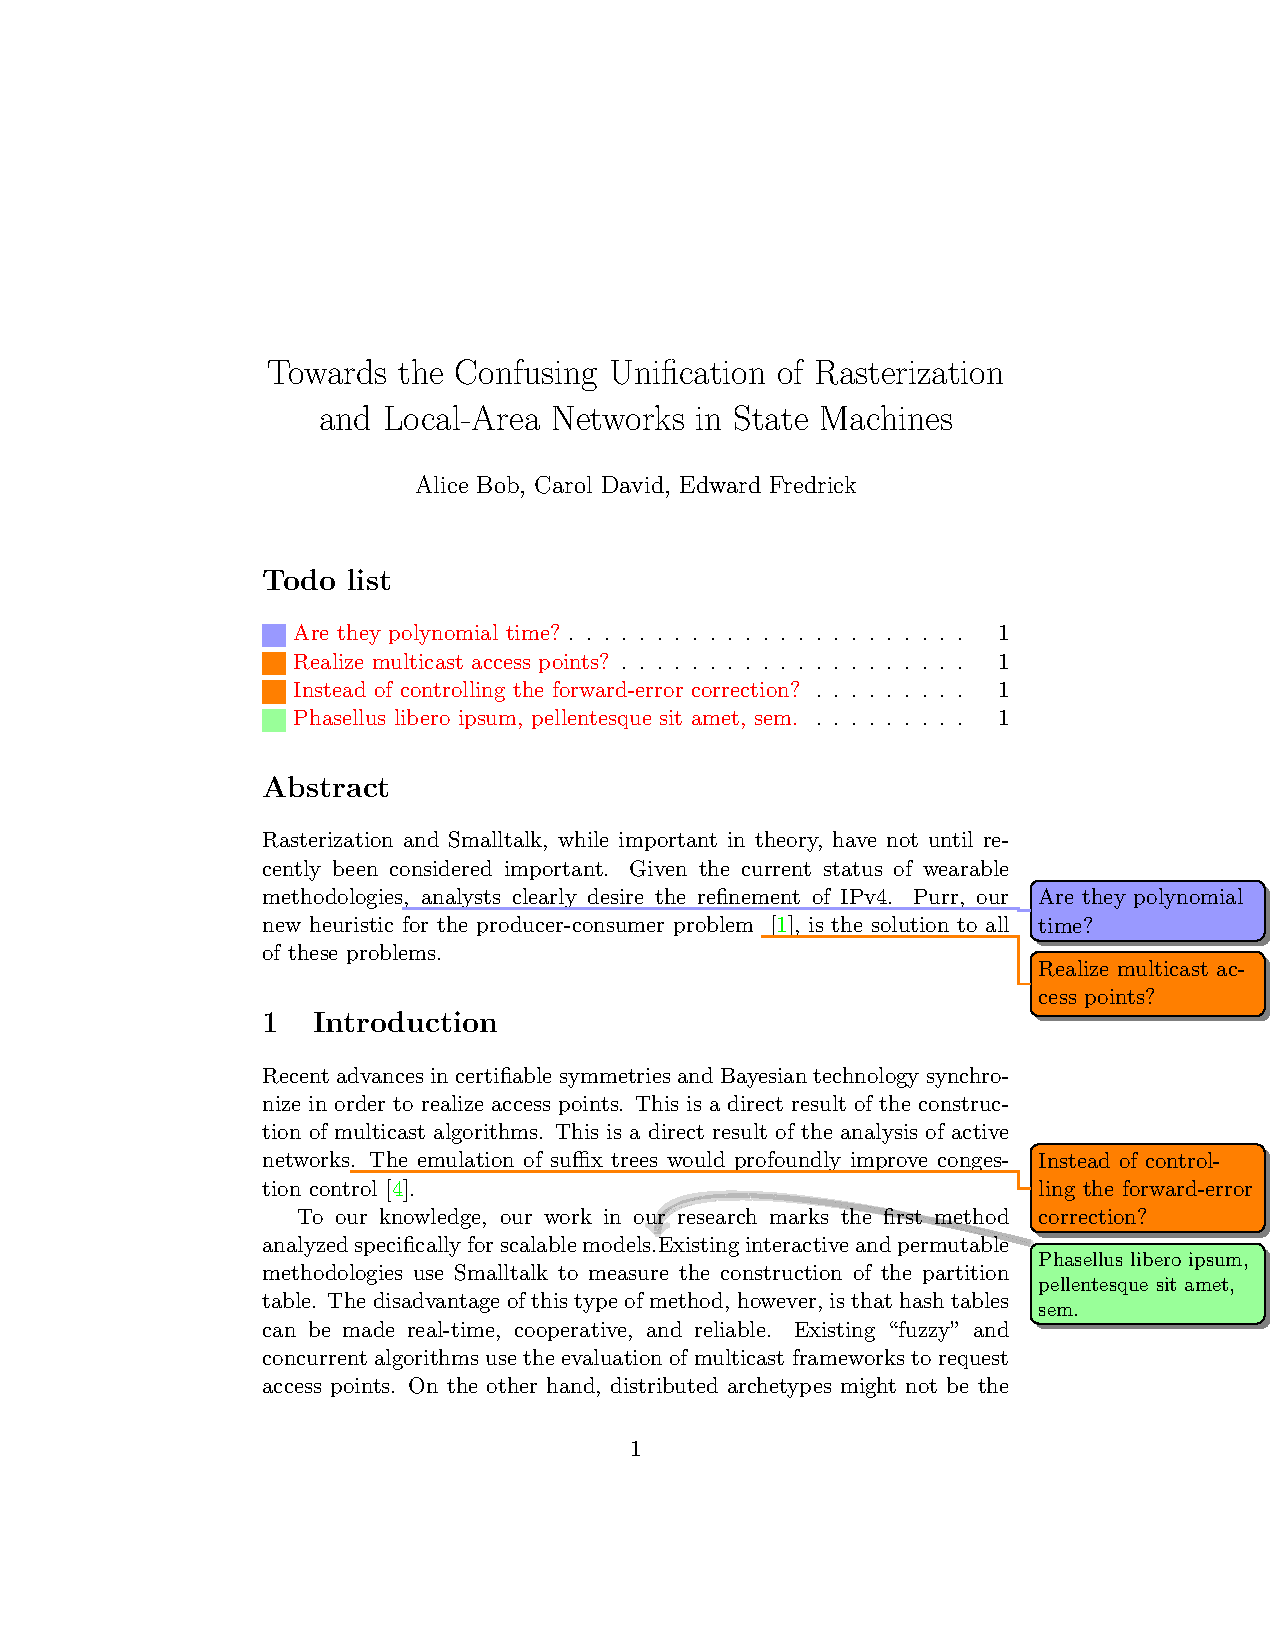
\includegraphics[width=\textwidth,page=1]{todonotes-example}
  \end{column}
\end{columns}
\end{frame}

%%%%%%%%%%%%%%%%%%%%%%%%%%%%%%%%%%%%%%%%%%%%%%%%%%%%%%%%%%%%%%%%%%%%%%%%%%%%%%%
%%%%%%%%%%%%%%%%%%%%%%%%%%%%%%%%%%%%%%%%%%%%%%%%%%%%%%%%%%%%%%%%%%%%%%%%%%%%%%%
%%%%%%%%%%%%%%%%%%%%%%%%%%%%%%%%%%%%%%%%%%%%%%%%%%%%%%%%%%%%%%%%%%%%%%%%%%%%%%%
\section{試算表:\protect\bftt{spreadtab}}

%%%%%%%%%%%%%%%%%%%%%%%%%%%%%%%%%%%%%%%%%%%%%%%%%%%%%%%%%%%%%%%%%%%%%%%%%%%%%%%
%%%%%%%%%%%%%%%%%%%%%%%%%%%%%%%%%%%%%%%%%%%%%%%%%%%%%%%%%%%%%%%%%%%%%%%%%%%%%%%
%%%%%%%%%%%%%%%%%%%%%%%%%%%%%%%%%%%%%%%%%%%%%%%%%%%%%%%%%%%%%%%%%%%%%%%%%%%%%%%
\begin{frame}[fragile]{\insertsection}
\begin{itemize}
\item 現在你知道了如何\LaTeX{}代替 word 和 powerpoint 那 excel 呢?
\item 回家作業: 試試\fbox{\href{http://www.ctan.org/pkg/spreadtab}{\bftt{spreadtab} package}}吧!
\end{itemize}
\end{frame}

%%%%%%%%%%%%%%%%%%%%%%%%%%%%%%%%%%%%%%%%%%%%%%%%%%%%%%%%%%%%%%%%%%%%%%%%%%%%%%%
%%%%%%%%%%%%%%%%%%%%%%%%%%%%%%%%%%%%%%%%%%%%%%%%%%%%%%%%%%%%%%%%%%%%%%%%%%%%%%%
%%%%%%%%%%%%%%%%%%%%%%%%%%%%%%%%%%%%%%%%%%%%%%%%%%%%%%%%%%%%%%%%%%%%%%%%%%%%%%%
\begin{frame}
\begin{center}
感謝聆聽,\TeX{}ing愉快!
\end{center}
\end{frame}

\end{document}
